\documentclass[thesis.tex]{subfiles}
\usepackage{multirow}
\usepackage{amsmath}
\usepackage{graphicx}
\usepackage{amssymb}
 
\begin{document}
\chapter{Theoretical Background}

\section{Standard Model}
The Standard Model (SM) of particle physics is a well-tested and successful model that describes the elementary particles and their interactions. 
It consists of a set of matter particles and force carriers, as well as the Higgs boson which gives mass to fundamental particles. 
All the SM particles and their properties are organized in Table 1. 
These particles are classified into two groups: fermions with half-integer spin, and bosons with integer spin.

\begin{table}[h]
\centering
\begin{tabular}{ |c|c|c|c|c|c|c|c|c|c| }
	\hline \hline
	\multicolumn{10}{ |c| }{Fermion: spin $\frac{1}{2}$ } \\
	\hline
		& \multicolumn{3}{c}{1st generation} & \multicolumn{3}{ |c| }{2nd generation} & \multicolumn{3}{ |c| }{3rd generation} \\
	\cline{2-10}
		& particle & charge & mass & particle & charge & mass & particle & charge & mass \\
	\hline
	\multirow{2}{*}{Lepton} & e            & $\pm$ 1    & 0.511 & $\mu$ & $\pm$ 1 & 0.511 & $\tau$ & $\pm$ 1 & 0.511 \\
	                                     &$\nu_e$  &  0              &  0          &$\nu_\mu$  &  0              &  0   &$\nu_\tau$  &  0              &  0    \\
	\hline
	\multirow{2}{*}{Quark}  &  u           &  $\pm \frac{2}{3}$     & 0.511 & c & $\pm  \frac{2}{3}$ & 0.511 & t   & $\pm  \frac{2}{3}$ & 0.511 \\
					    & d           &  $\pm \frac{1}{3}$     & 0.511 & c & $\pm  \frac{1}{3}$ & 0.511 & t   & $\pm  \frac{1}{3}$ & 0 \\ 
	\hline \hline
	\multicolumn{10}{ |c| }{Gauge Boson: spin 1 } \\
	\hline
	Partile  &  \multicolumn{3}{c|}{Interaction}  &  \multicolumn{3}{c|}{ Mass }  &   \multicolumn{3}{c|}{ Charge } \\
	 \hline
	 $\gamma$ &  \multicolumn{3}{c|}{EM}  &  \multicolumn{3}{c|}{ 0 }  &   \multicolumn{3}{c|}{ 0 } \\
	 \hline
	 W &  \multicolumn{3}{c|}{Weak}  &  \multicolumn{3}{c|}{ $\pm$ 1 }  &   \multicolumn{3}{c|}{ 80 } \\
	 \hline
	 Z &  \multicolumn{3}{c|}{Weak}  &  \multicolumn{3}{c|}{ 0 }  &   \multicolumn{3}{c|}{ 90 } \\
	 \hline
	 g &  \multicolumn{3}{c|}{Strong}  &  \multicolumn{3}{c|}{ 0 }  &   \multicolumn{3}{c|}{ 0 } \\
	 \hline \hline
	 \multicolumn{10}{ |c| }{Higgs Boson: spin 0 } \\
	 \hline
	 H &  \multicolumn{3}{c|}{-}           &   \multicolumn{3}{c|}{ 125 }  &   \multicolumn{3}{c|}{ 0 } \\
	 \hline
	                                     
\end{tabular}
\end{table}

The SM was built within a framework known as Quantum Field Theory (QFT), which provides the mathematical tools to describe the subatomic particles using theories that are consistent both with quantum mechanics and special relativity. 
In QFT, particles are represented by excitations of quantum field. 
The dynamics and interactions of the particles are described by the Lagrangian formalism using the Lagrangian density $\mathcal{L}$. \\

Fundamental fermions are the basic building blocks of matter. 
They occur in two varieties: leptons that do not undergo strong interaction, and quarks that participate in the strong interactions. 
There has been observed three generations of leptons and quarks, each consisting of a charged lepton (e, mu, tao), a neutral neutrino (nu, nu, nu) which is almost massless and interacts only via the weak force and gravity, an up-type quark (u,c,t) with 2/3 electric charge, and a down-type quark (d,s,b) with -1/3 electric charge. 
Each of these fermions has an associated anti-particle with the same mass but with opposite charge. \\

There are four fundamental forces of nature: the strong interaction, the weak interaction, the electromagnetic force, and gravity. 
Each of these forces, except gravity, is mediated by its corresponding gauge bosons. 
The SM is a gauge quantum field theory based on the symmetry group 
	\begin{equation}
		SU(3) \otimes SU(2) \otimes U(1)_Y,
	\end{equation}
 where, SU(2)$\otimes$U(1)$_Y$ is the symmetry of electroweak interactions, and SU(3) group describes the symmetry of strong interactions. 
The SU(2) group has three gauge bosons $W_{i, i = 1,2,3}^{\mu}$, and the U(1)$_Y$ group has one gauge boson $B^{\mu}$. 
The linear combination of these gauge bosons form the physical particles: photon ($\gamma$), $W^{\pm}$ and Z. 
The photon is a massless vector boson which has two polarizations, and it is the force carrier of the electromagnetic interactions. 
The $W^+$/$W^{-}$ and Z bosons are massive vector bosons that mediate the weak force. 
The gauge boson of the SU(3) group is the gluon, which is a massless particle that carries color charge and couples to quarks and other gluons. \\
 
The Lagrangian of the SM can be decomposed into four terms: 
	\begin{equation}
		\mathcal{L} =  \mathcal{L}_{Gauge} + \mathcal{L}_{kin} + \mathcal{L}_{Y} + \mathcal{L}_{H}
	\end{equation}
The first term is the kinetic term of the SM gauge bosons:
	\begin{equation} 
		\mathcal{L}_{Gauge} = -\frac{1}{4}B_{\mu\nu} B^{\mu\nu} - \frac{1}{4}F_{\mu\nu}^a F^{a \mu\nu} - \frac{1}{4} G_{\mu\nu}^A G^{A \mu\nu}
	\end{equation}
where a = 1,2,3; and A = 1 ... 8. The field strengths are:
	\begin{equation}
		\begin{array}{c c l}
			B_{\mu\nu} & = & \partial_\mu B_\nu - \partial_\nu B_\mu \\
			F_{\mu\nu}^a &=&  \partial_\mu W_\nu^a - \partial_\nu W_\nu^a + g \epsilon^{abc}W_\mu^b W_\nu^c \\
			G_{\mu\nu}^A &=& \partial_\mu G_\nu^A - \partial_\nu G_\nu^A + g_s f^{ABC}G_{\mu}^B G_{\nu}^C 
		\end{array}
	\end{equation}
The Levi-Civita tensor $\epsilon^{abc}$ and the Gell-Mann tensor $f^{ABC}$ are the structure constants of the SU(2) and SU(3) group, respectively. 

			
	

The second term  of \ref{eq:SML} describes the fermion fields and their gauge interactions. 
Fermion fields are classified into left-chiral and right-chiral states according to their chirality under Lorentz transformations. 
The left-chiral states are SU(2) doublets, while the right-chiral states are singlets:
	\begin{equation}
		\begin{array}{cl}
		\text{Lepton doublet}: & L = \left( \begin{array}{c} \nu_i \\ e_i \end{array} \right)_L \\
		\text{Lepton singlet}:  & \bar{l}_{R} \\
		\text{Quark doublet}:  & Q =  \left( \begin{array}{c} u \\ d \end{array} \right)_L \\
		\text{Quark singlet}:    & \bar{u}_{R}, \bar{d}_{R}
		\end{array}
		\label{eq:SML}
	\end{equation}
The $\mathcal{L}_{kin}$ term has the form: 
	\begin{equation}
		\mathcal{L}_{kin} =  \sum_{i}^3 \left( L_i^\dagger \sigma^\mu D_\mu L_i +
									\bar{l}_i^\dagger \sigma^\mu D_\mu \bar{l}_i + 
									Q_i^\dagger \sigma^\mu Q_\mu L_i +
									\bar{u}_i^\dagger \sigma^\mu D_\mu \bar{u}_i +
									\bar{d}_i^\dagger \sigma^\mu D_\mu \bar{d}_i \right)
	\end{equation}
where $i$ is the generation index. $D_\mu$ is the covariant derivative, which has the form: 
	\begin{equation}
		D_\mu = (\partial_\mu + i g`YB_\mu + i g \sigma_a W_\mu^a + ig_s \lambda_b G_\mu^{b} ).
	\end{equation}
$\lambda_b$ are the eight Gell-Mann matrices that generate the SU(3) group.  \\

The second term of \ref{eq:SML} is the kinetic term of the SM gauge bosons:
	\begin{equation} 
		\mathcal{L}_{Gauge} = -\frac{1}{4}B_{\mu\nu} B^{\mu\nu} - \frac{1}{4}F_{\mu\nu}^a F^{a \mu\nu} - \frac{1}{4} G_{\mu\nu}^A G^{A \mu\nu}
	\end{equation}


 
The gauge bosons are required to be massless in order to reserve gauge invariance. 
This is the case for gluons and photons. However, the observed W and Z bosons are heavy particles, which implies that the symmetry is somehow broken. 
A mechanism named ?spontaneous symmetry breaking? [] is introduced to give masses to the W and Z bosons while preserve the renormalizability of the theory. 
The idea is that the ground state of the theory is not invariant under the symmetry transformation.
This is achieved by adding a complex SU(2) doublet scalar field, which is know as the Higgs field, to the SM Lagrangian. 
The potential of the Higgs field has the form: 
	\begin{equation}
		V(\phi) = \mu^2\phi^*\phi + \lambda(\phi^*\phi)^2,
	\end{equation}
provided $\mu^2 <$ 0 this potential has minimum: 
	\begin{equation}
		v = \sqrt{ -\mu^2/\lambda}.
	\end{equation}
There is an infinite number of ground state lying on a ring described by $\phi^*\phi = - \mu^2/\lambda$. 
Making a choice of the ground state will spontaneously break the symmetry, since a gauge transformation will take the system to a different vacuum state. 
Adopting the unitary gauge, we choose the ground state to be along the real axis of the lower component of the doublet.
The Higgs field can be expanded around the vacuum as:
	\begin{equation}
		<\phi> = \frac{1}{\sqrt{2}} \left( \begin{array}{c} 0\\v+H \end{array} \right),
	\end{equation}
Substituting the Higgs field to the kinetic term $(D_\mu \phi)^\dagger(D^\mu\phi)$, where:
	\begin{equation}
		D_\mu = \partial + i\frac{g}{2}\left(  \begin{array}{c} W_\mu^3   \sqrt{2}W_\mu^- \\ \sqrt{2}W_\mu^+  -W_\mu^3 \end{array} \right) + i\frac{g`}{2}B_\mu, 
	\end{equation}
we find:
	\begin{equation}
		(D_\mu \phi)^\dagger(D^\mu\phi) = \frac{1}{2}(\partial H)^2 + \frac{g^2v^2}{4}W^{+\mu}W_{\mu}^- + \frac{v^2}{8}(gW_\mu^3 - g`B_\mu)^2.
	\end{equation}
Define
	\begin{equation}
	\begin{array}{c}
		Z_\mu = cos\theta_W W_\mu^3 - sin \theta_W B_\mu \\
		A_\mu = cos\theta_W B_\mu + sin\theta_W W_\mu^3
	\end{array}
	\end{equation}
the kinematic term can be rewritten as:
	\begin{equation}
		(D_\mu \phi)^\dagger(D^\mu\phi) = \frac{1}{2}(\partial H)^2 + \frac{g^2v^2}{4}W^{+\mu}W_{\mu}^- + \frac{v^2g^2}{8cos^2\theta_W}Z_\mu Z^\mu + 0A_\mu A^\mu
	\end{equation}
We recognize the second and third terms as the mass term of W and Z bosons. On the other hand, leptons and quarks gain mass through coupling to the Higgs particle.  \\

An extensive set of experiments has been made in the past few decades to test the SM. 
The W and Z bosons were discovered in 1983 at CERN. The top quark, which is the heavist quark, were observed in 1995 at Fermilab. 
In 2012, the CMS and ATLAS experiment at CERN announced the observation of Higgs bosons, and this discovery completed the last missing piece of the SM.  
The SM predictions agree well with the observed data in a wide range of experiments. 
For example, Figure \ref{fig1-1} shows the consistency of the predicted cross-section of the SM processes in LHC and the measurements made by the CMS experiment.
	\begin{figure*}[hbtp]
		\centering
	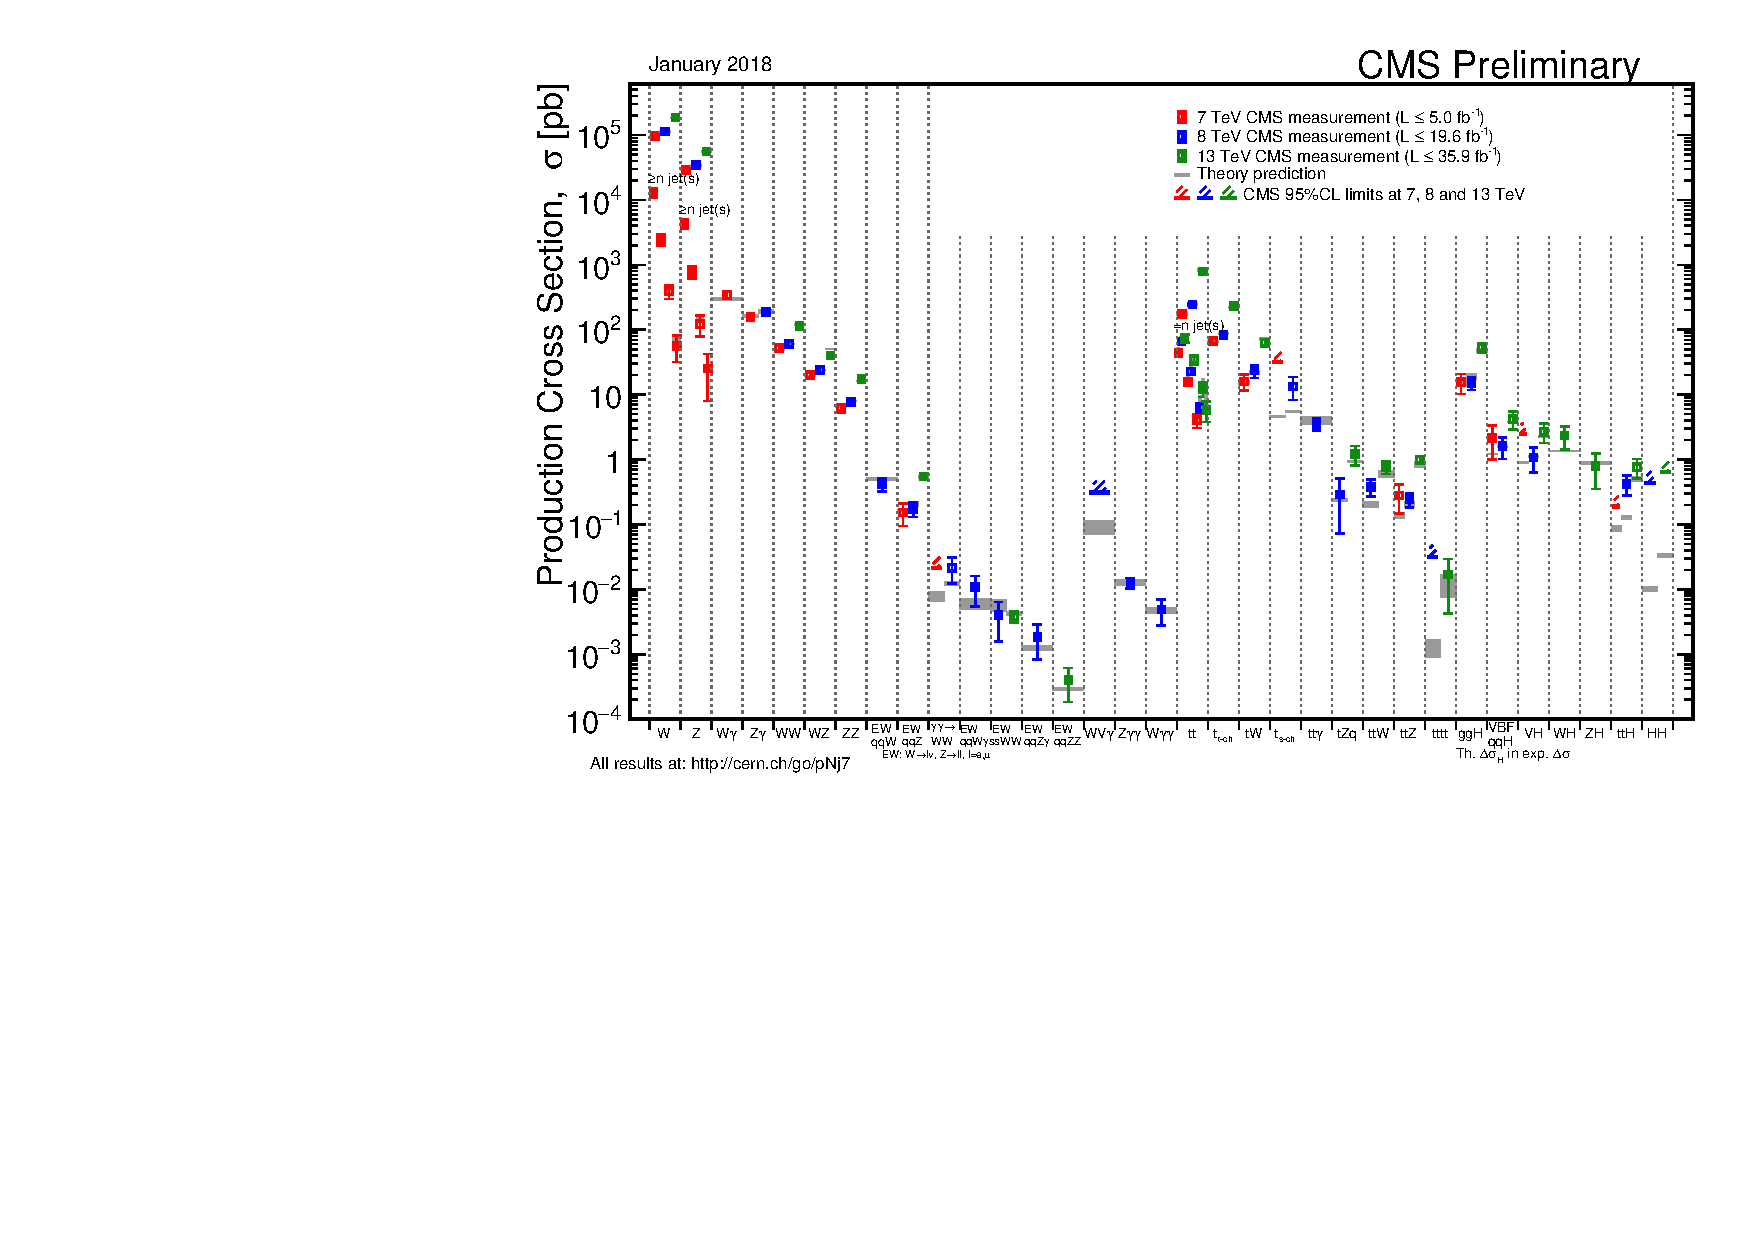
\includegraphics[width=0.6\textwidth]{plot/SigmaNew_v0.pdf}
	\end{figure*}
	

\section{Problems of the Standard Model}
Although the SM is remarkably successful at explaining a wide range of phenomena, it does leave many questions unanswered. 
One major problem is the omission of the gravity - the most familiar fundamental force. 
Phenomena at large scale can be well described by the general relativity, however, there is not yet a satisfactory theory which can incorporate the gravity at subatomic scale. 
Therefore the SM is believed to be a low-energy approximation of a theory existing at the $10^{19}$ GeV Planck scale, the energy at which the gravity is comparable to the other forces and can no longer be ignored.\\

Another outstanding problem of the SM is the lack of explanation for dark matter (DM), so named because it doesn't undergo electromagnetic interactions and thus is invisible to normal matter. The dark matter was discovered through the measurement of velocity dispersion and rotation curves of the galaxies, whose results indicated that the luminous matter cannot explain the observed curves on its own and some invisible matter is needed to account for. Measurements show that roughly 80\% of the matter in the universe is made of dark matter. Despite the extensive experimental efforts of searching for the DM, we still know little about the nature of the DM and its interactions with the normal matter described by the SM. \\

Besides the lack of particle candidates for the gravity and DM, there are some observations that the SM  cannot explain. One of these mysteries is the large discrepancy between the electroweak and Planck scale, which is known as the hierarchy problem. The Higgs mass is measured to be 126 GeV, $10^{17}$ lower than the Planck scale. The physical Higgs mass is a combination of the tree-level bare mass and high order corrections. Because the loop corrections of the Higgs mass contains quadratic divergences, its bare mass has to cancel the corrections with an accuracy up to 26 digits leaving a small mass at electroweak scale. This unnatural cancellation is called "fine tuning problem", and it suggests the appearance of new physics which can stabilize the Higgs mass. \\

Due to these issues, the SM is considered as an incomplete theory, and many new theories beyond the SM have been introduced to incorporate the unexplained features in the SM. 


\section{Supersymmetry}

Supersymmetry (SUSY) is a favored extension of the SM that provides solutions for many of the problems of the SM. 
It unifies the description of forces and matter by inducing a symmetric transformation between bosons and fermions. 
SUSY doubles the number of particles by paring each of the SM particles with a SUSY partner ? each fermion has a bosonic partner named sfermion and each gauge boson has a fermionic partner named gaugino. 
The SM particle and its superpartner has the same quantum number except the spin. 
Table 2 lists the SM particles and the corresponding superpartners. 
In the loop corrections to the Higgs self energy, the contributions from fermions and bosons cancel with each other, leaving a light Higgs mass at the electroweak scale. This is illustrated in Fig. 7. \\

Constructing a supersymmetric Lagrangian in the 4-dimensional spacetime with brutal force can be very difficult and tedious. 
The introduction of superspace greatly simplified the calculations. 
The superspace extends the usual spacetime coordinates with two fermionic (or Grassmannian) coordinates. 
Points in superspace have coordinates:
     \begin{equation}
	(x^\mu, \theta, \theta^\dagger)
     \end{equation}
where $x^\mu$ are space-time coordinates and $\theta$, $\theta^\dagger$ are anti-commuting Grassmann variables.\\

A supersymmetry transformation performs a rotation in the superspace.
Such transformations are generated by operator Q, which is called the supercharge.  
The operator Q acts on the states, turning a fermionic component into a bosonic component, and vice verse, as: 
      \begin{equation}
        Q| Boson > = | Fermion>,  Q|Fermion> = |Boson>.
      \end{equation} 

The supercharge itself is a spinor, so its hermitian conjugate $Q^\dagger$ is also a symmetry generator. 
They satisfy the following commutation relations:
    \begin{equation}
     \{Q_a, Q_{\dot{a}}^\dagger \} = (\sigma^\mu})_{a\dot{a}} P_\mu,
     \end{equation} 
    \begin{equation}
     \{Q_a, Q_b \} = 0,
     \{Q_{\dot{a}}^\dagger, Q_{\dot{b}}^\dagger \} = 0,
      \end{equation} 
      \begin{equation}
     [Q_a, P_\mu] = 0,  [Q_{\dot{a}}^\dagger,  P_\mu] = 0
    \end{equation} 
where $P_\mu = i\partial_\mu$ is the momentum operator. 
The first anti-commutation relation in equation () indicates that ?...... \\

The field content is grouped into supermultiplets that contain the SM fields and superpartiners. 
Supermultiplets are described by functions over the superspace, which are referred to as superfield. 
A chiral superfield can be expressed by expansion in Grassmann variables as:
    \begin{equation}
    \Phi(x, \theta, \theta^\dagger) = \phi(x) + \theta\psi(x) + \frac{1}{2}\theta\theta F(x) + (space-time \ derivatives\ acting\ on\ \phi \ and \ \psi )
    \end{equation}
 where $\phi$ is a complex scalar field, $\psi$ is a left-chiral spinor, and $F(x)$ is an auxiliary field. 
 The  auxiliary is ?.. \\
    
 To write down SUSY Lagrangians that contain gauge interactions, we also need vector superfields. 
 A general form of a vector superfield in the Wess-Zumino gauge is:
    \begin{equation}
   V = - \theta\sigma^\mu\bar{\theta}V_\mu(x) + i\theta^2\bar{\theta}\bar{\lambda}(x) - i\bar{\theta}^2\theta\lambda(x) + \frac{1}{2}\theta^2\bar{\theta}^2D(x)
   \end{equation}
where $V_\mu(x)$ is the gauge field, $\lambda(x)$ and $\bar{\lambda}$ are gauginos, and D(x)....\\

Super potential? Lagrangian? MSSM ?

\subsection{Supersymmetry Breaking}
As mentioned before, the quadratic divergence of the Higgs mass arising from SM loop can be exactly cancelled by the contribution from SUSY partners when the masses of all states in a supermultiplet are degenerate. 
However, any partners with the same mass of leptons or light quarks should have been observed. 
Therefore supersymmetry must be a broken symmetry at low energy scale if it is realized in nature. 
In order to maintain the good ultraviolet behaviour of the supersymmetry while split the mass between the SM particles and their SUSY partners, a soft symmetry breaking is considered. 
The idea is that supersymmetry is unbroken at some high energy scale at which the exact SUSY is preserved. 
At low energy scale, the supersymmetry breaking takes place, allowing the SUSY particles to obtain heavier mass than their SM partners. \\

Soft supersymmetry breaking terms can arise as an effective description of  the spontaneous supersymmetry breaking, i.e. the Lagrangian is invariant under supersymmetric transformations but the vacuum state is not. 
The spontaneous supersymmetry breaking happens when the supercharges do not annihilate the vacuum, i.e., 
    \begin{equation}
	Q|0> =\ = 0
    \end{equation}
Using the commutation relation (1.) of the supercharges, we can write the Hamiltonian as
	 \begin{equation}
	H = P^0 = \frac{1}{4}(Q_1bar{Q_i} + bar{Q_i}Q_1 + Q_2 bar{Q_2dot} + bar{Q_2dot} Q_2}
	  \end{equation}
which has positive vacuum expectation value (VEV) when SUSY is spontaneous broken, i.e.
	 \begin{equation}
	<0| H |0>  > 0.
	\end{equation}

SUSY breaking within the MSSM is not easy, because it predicts SUSY particles that are lighter than their SM partners. 
The way out is to assume the existence of a hidden sector that is uncharged under the SM gauge group. 
The SUSY breaking originates in the hidden sector and communicate to the visible MSSM sector by a set of messenger fields. 
The messenger sector transmits the SUSY breaking via loop corrections, allowing the SUSY particles to become massive. 
There are several well studied mechanism for mediating the SUSY breaking to the visible sector, including gravity mediation, gauge mediation and anomaly mediation. 
The search presented in this thesis is motivated by the gauge mediated SUSY breaking (GMSB). 

The GMSB mechanism assume that the messenger sector couple to the visible sector via flavor-blind gauge interactions. 
Suppose the hidden sector has some supermultiplet S which has VEV $<F>$, where F is the auxiliary field of S. 
A set of messenger fields ${\Phi_I, \bar{\Phi}_I}$ couple to the hidden sector via interaction term:
	 \begin{equation}
	W = \Sum_I y_I S \Phi_I \bar{\Phi}_I.
	\end{equation}
If <F> is non-zero, mass splittings are generated in the messenger sector. 
The messenger fields are charged under the SM gauge. 
Therefore the SUSY breaking is mediated from the hidden sector to the visible sector through gauge interaction. A scheme of the gauge mediation is shown in Figure X. 

picture

The gauginos become heavier due to the radiative corrections from messenger particle loops, as illustrated in the Feynman diagram of Figure X. 
 	diagram

The resulting gaugino and sfermion mass have the form

	$M_\lambda \sim $ 
	
	$M_sf \sim$

\subsection{Phenomenology of General Gauge mediation Supersymmetry}

According to the Goldstone's theorem, for every global symmetry with spontaneous breaking there exist a massless Nambu?Goldstone boson. 
Similar to the goldstone boson, spontaneous SUSY breaking gives rise to a massless goldstino. 
When SUSY is imposed as a local symmetry, the goldstino is absorbed by the gravitino, becoming the longitudinal component of the gravitino. 
The gravitino mass is:\\
	$m_2/3 \sim <F>/M_PL$
	\\
The mediation scale could be low, making the gravitino very light. 
In gauge-mediated SUSY, the lightest supersymmetry particle (LSP) is the gravitino. 
All the heavier SUSY particles will decay cascade to the gravitino. 



\end{document}


